% !TeX document-id = {1ea8a8bb-daca-4a90-a524-965e19928468}
% !TEX spellcheck = en-US
% !BIB TS-program = biber
\documentclass[10pt,a4paper]{article}
\usepackage[english]{babel}
\usepackage{ragged2e}
\usepackage{float}
\usepackage[style=apa, backend=biber,natbib]{biblatex}
\DeclareLanguageMapping{english}{english-apa}
\addbibresource{refs.bib}
\bibliography{refs}  
\usepackage[utf8]{inputenc}
\usepackage[T1]{fontenc}
\usepackage{amsmath}
\usepackage{amsfonts}
\usepackage{amssymb}
\usepackage{graphicx}
\usepackage{pgfgantt}
\author{Yapi Donatien Achou}
\title{Implementation of Skaiwatch predictive maintenance platform}
\begin{document}
\maketitle

\section{Motivation for Skaiwatch predictive maintenance platform}
Skaiwatch as a predictive maintenance platform aims at bringing values to our customers by automating machine diagnostic and prognostic. The former specifies the type of faults incur by a machine, while the latter is concerned with the severity of the fault type, and is directly tied to the remaining useful life of an asset. Skaiwatch follows the vision of Karsten Moholt founder, which is continuous improvement, through innovation for customers satisfaction.
\justify
The goal is to implement a web based application available any where on any device. The application is a suit of software that facilitates the predictive maintenance pipeline through automation, from  diagnostic, prognostic, remaining useful life estimation, recommendations, reporting to maintenance planing. The technology used in this project is mature and well established and is based on signal processing, statistics and probability, machine leaning, mathematical optimization, and web technology.
\justify
On the customers view points, the benefits are invaluable. The obvious one is cost saving. By knowing the current and future health state of a machine, the customers are immune to sudden breakdown or downtime, which could alt production and incur significant financial or even human cost. The previous point leads to confidence in the reliability of machines and is essential for machine based production. This allows business partners to rely on each other and creates an efficient and serene business atmosphere.
\justify
For Karsten Moholt view point, Skaiwatch is the response to continuous innovation in order to maintained its competitive advantage and avoid obseleteness.
\section{Current status and future work}
\label{sec:next}
Currently, we have worked on one external and two internal projects, that resulted in understanding and formulating a predictive maintenance problem, presenting a solution through a demo web application, that automates machine faults detection. 
\justify
The next step is to set a time line, plan and execute a project for a complete predictive maintenance platform, which we called Skaiwatch. The latter is centered on the following key Item:
\begin{enumerate}
	\item An automated vibration tool box for bearing fault detection
	\item An automated tool box for non rotating machines
	\item A time series analysis tool box 
	\item An automated reporting application for recommendations, machines status and maintenance planning
\end{enumerate}
\section{Project founding and project Plan}
\subsection{Project founding scheme}
Implementation of the Skaiwatch predictive platform will be founded by the Research Council of Norway industrial PhD scheme. The latter finances 50$\%$ of the project cost and requires 

\begin{enumerate}
	\item A PhD candidate
	\item A project manager
	\item A project administrator
\end{enumerate}
The scheme allows companies to collaborate with Universities for a research based project that brings values into private sector companies. The duration of the project is between 3 to 4 years.
\justify
The scheme does not require companies to directly contribute the remaining $50\%$ of the project cost in financial cost, but in man hours (Salary of the project participant). The application process is simple and 3 weeks after submitting the application a feedback is given. 
\begin{figure}[H]
	\centering
	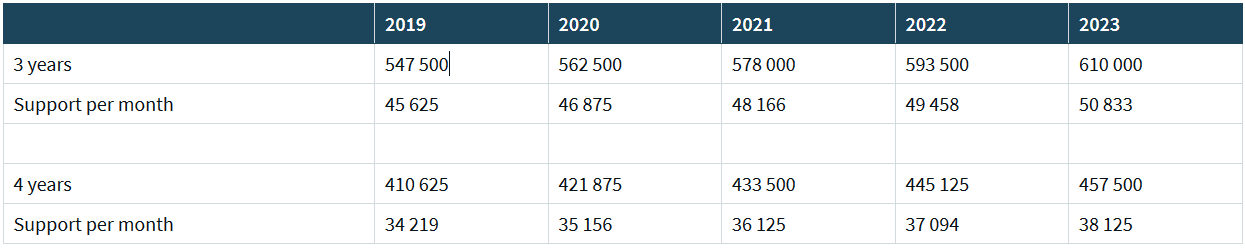
\includegraphics[width=1.\linewidth]{table}
	\caption{}
	\label{fig:table}
\end{figure}

Figure \ref{fig:table} shows the founding provided by the research council of Norway per year for the Industrial Phd scheme.
\subsection{Tentative project plan} 
\clearpage
\subsubsection{ Automated vibration analysis tool box}
\begin{ganttchart}[
	vgrid,title/.style={fill=teal, draw=none},title label font=\color{white},bar/.append style={fill=blue!50},
	group/.append style={draw=black, fill=green!50},
	]{1}{12}
	\gantttitle{January 2020-December 2020}{12} \\
	\gantttitlelist{1,...,12}{1} \\
	\ganttgroup{Group1: Literature and course}{1}{5}\\
	%\ganttgroup{Group 1}{1}{7}[style={inner color=blue}] \\
	\ganttbar{Course 1: Statistical learning UIB}{1}{5} \\
	\ganttbar{Fourier analysis literature survey}{2}{3}\\
	\ganttbar{Wavelet and Hilbert Huang transform (HHT) literature survey}{3}{4}\\
		\ganttgroup{Group2: Software development}{5}{12}\\
	\ganttbar{Python Implementations of Fourier, Wavelet and HHT}{5}{8}\\
%	\ganttbar{Web interface for Fourier, wavelet and HHT}{5}{8}\\
	\ganttbar{First research paper}{8}{12}
\end{ganttchart}



%blala (\cite{albrecht1986}) and then (\cite{albrecht1986})


%\bibliographystyle{apacite}
%%\addcontentsline{toc}{chapter}{\bibname}
\printbibliography
\end{document}